\documentclass[11pt]{article}

\usepackage{float}
\usepackage{hyperref}
\usepackage{graphicx}
% formatting
\usepackage{verbatim}
\usepackage{moreverb}
\usepackage{minted}
\usepackage{parskip}
\usepackage{amsmath}
\usepackage[listings]{tcolorbox}
\usepackage{enumerate}
\let\verbatiminput=\verbatimtabinput
\def\verbatimtabsize{4\relax}

\newcommand{\RepoRootPath}{fpga\_labs\_fa19}

\tcbset{
texexp/.style={colframe=black, colback=lightgray!15,
         coltitle=white,
         fonttitle=\small\sffamily\bfseries, fontupper=\small, fontlower=\small},
     example/.style 2 args={texexp,
title={Question \thetcbcounter: #1},label={#2}},
}

\newtcolorbox{texexp}[1]{texexp}
\newtcolorbox[auto counter]{texexptitled}[3][]{%
example={#2}{#3},#1}

\setlength{\topmargin}{-0.5in}
\setlength{\textheight}{9in}
\setlength{\oddsidemargin}{0in}
\setlength{\evensidemargin}{0in}
\setlength{\textwidth}{6.5in}

% Useful macros

\newcommand{\note}[1]{{\bf [ NOTE: #1 ]}}
\newcommand{\fixme}[1]{{\bf [ FIXME: #1 ]}}
\newcommand{\wunits}[2]{\mbox{#1\,#2}}
\newcommand{\um}{\mbox{$\mu$m}}
\newcommand{\xum}[1]{\wunits{#1}{\um}}
\newcommand{\by}[2]{\mbox{#1$\times$#2}}
\newcommand{\byby}[3]{\mbox{#1$\times$#2$\times$#3}}


\newenvironment{tightlist}
{\begin{itemize}
 \setlength{\parsep}{0pt}
 \setlength{\itemsep}{-2pt}}
{\end{itemize}}

\newenvironment{titledtightlist}[1]
{\noindent
 ~~\textbf{#1}
 \begin{itemize}
 \setlength{\parsep}{0pt}
 \setlength{\itemsep}{-2pt}}
{\end{itemize}}

% Change spacing before and after section headers

\makeatletter
\renewcommand{\section}
{\@startsection {section}{1}{0pt}
 {-2ex}
 {1ex}
 {\bfseries\Large}}
\makeatother

\makeatletter
\renewcommand{\subsection}
{\@startsection {subsection}{1}{0pt}
 {-1ex}
 {0.5ex}
 {\bfseries\normalsize}}
\makeatother

% Reduce likelihood of a single line at the top/bottom of page

\clubpenalty=2000
\widowpenalty=2000

% Other commands and parameters

\pagestyle{myheadings}
\setlength{\parindent}{0in}
\setlength{\parskip}{10pt}

% Commands for register format figures.

\newcommand{\instbit}[1]{\mbox{\scriptsize #1}}
\newcommand{\instbitrange}[2]{\instbit{#1} \hfill \instbit{#2}}
\newcommand{\itwos}{I\textsuperscript{2}S}

\begin{document}

\def\PYZsq{\textquotesingle}
\title{\vspace{-0.4in}\Large \bf EECS 151/251A FPGA Lab 4:\\FPGA Memories, Audio\vspace{-0.1in}}

\author{Prof. John Wawrzynek \\
TAs: Quincy Huynh, Tan Nguyen \\ Department of Electrical Engineering and Computer Sciences\\
College of Engineering, University of California, Berkeley}
\date{}
\maketitle

\section{Before You Start This Lab}\label{sec:begin}
You should run \verb|git pull| in \verb|fpga_labs_sp20| to get the latest files for this lab.

You should also review the lecture slides on Finite-State Machine. For additional resource, take a look at \href{http://inst.eecs.berkeley.edu/~eecs151/sp20/files/verilog/verilog\_fsm.pdf}{verilog\_fsm.pdf}

In this lab, we cover FPGA memories and audio. We will learn to how to leverage the memory resource on FPGA for data storage. In addition, we will build circuits that play musical tones by implementing an I2S protocol to interface with an off-chip DAC (Digital-to-Analog) of Pmod I2S module. If you do not have a Pmod I2S module around when you start working on this lab, please notify a TA.

\section{FPGA Memories}

Recall that in Lab 2, we explored different types of resource on our FPGA. Besides the LUTs and FFs for logic implementation, the FPGA also offers Memory LUTs (SLICEM) and Block RAMs for on-chip data storage. This brings many benefits as the read/write accesses to those memories are fast and predictable, unlike off-chip memory accesses. Think of it like a cache, with the downside that it is much harder to use than a cache since you have to manually manage data read and write yourself (but the good news is you can tailor the data reuse to your own application's memory access pattern). The density of those memory blocks also reduces the register pressure when you require a large number of state elements. For the purpose of this lab, we want to use the memories to provide data to our digital circuits to perform certain tasks.

Take a look at the file \verb|lib/EECS151.v|. Besides the REGISTER modules, we have some memory modules. There are two types of memory that we should pay attention for now: \textbf{Asynchronous Read/Synchronous Write} Memory, and \textbf{Synchronous Read/Synchronous Write} Memory. The former retrieves read data immediately, while the latter gets the data at the next clock cycle, hence read takes one cycle for Synchronous Read Memory. Both of them require one clock cycle for write. The Asychronous Read Memory typically gets mapped to Distributed RAMs on FPGA (Memory LUTs/LUTRAMs), while the Synchronous Read Memory is mapped to BRAMs. Additionally, we also have ROM-style memories for read-only data storage. Using ROMs also yields simpler control logic if you don't do any memory updates.

The memory are declared as an array of \verb|reg| nets as follows.

\begin{minted}[tabsize=2]{verilog}
(* ram_style = "block" *) reg [DWIDTH-1:0] mem [DEPTH-1:0];
\end{minted}

Depending on how you write your Verilog code that makes use of this \verb|reg|, the Synthesis tool will infer this \verb|reg| as either a bunch of separate registers or some form of memory block(s). Certain vendors adopt some specific coding style or synthesis attributes that gives hints to the tools to map your hardware nets to which FPGA resources. Here, the attribute \verb|ram_style = "block"| tells Vivado synthesis that we want to map this \verb|reg| to Block RAMs. Normally, we just let the tools to figure out what resources are best to use to create optimal designs. In some cases, the synthesis attributes gives some flexibility for us to force the tools to do what we want. Note that those attributes or coding styles may not apply from one vendor tool to another.
If you are interested to learn more, you should definitely take a look at \href{https://www.xilinx.com/support/documentation/sw_manuals/xilinx2019_2/ug901-vivado-synthesis.pdf}{Vivado Synthesis Guide}, Chapter 2 and 4.
To make it easier for you to use memory blocks, we have those defined in \verb|lib/EECS151.v|, and they are guaranteed to synthesize to memory blocks by Vivado.

We can initialize the content of our memories with the following Verilog constructs.

\begin{minted}[tabsize=2]{verilog}
initial begin
    if (MEM_INIT_HEX_FILE != "") begin
		    $readmemh(MEM_INIT_HEX_FILE, mem);
    end
    else if (MEM_INIT_BIN_FILE != "") begin
		    $readmemb(MEM_INIT_BIN_FILE, mem);
    end
end
\end{minted}

The Verilog code looks for a memory initialization file \verb|mif| to initialize the content of \verb|mem|. If the numeric data of the \verb|mif| file is in hex format, use \verb|$readmemh|, otherwise if it is in binary format, use \verb|$readmemb|. This works for both Bitstream Generation and Simulation too.

Here is another method to create an asynchronous ROM or a look-up table.

\begin{minted}[tabsize=2]{verilog}
module rom (input [2:0] address, output reg [11:0] data);
  always @(*) begin
    case(address)
      3'd0: data = 12'h000;
      3'd1: data = 12'hFFF;
      3'd2: data = 12'hACD;
      3'd3: data = 12'h122;
      3'd4: data = 12'h347;
      3'd5: data = 12'h93A;
      3'd6: data = 12'h0AF;
      3'd7: data = 12'hC2B;
    endcase
  end
endmodule
\end{minted}

Depending on the size of your data, you may want to pick the most convenient method for you. For this and later labs, please use the memory modules declared in \verb|lib/EECS151.v| whenever you want to instantiate a memory block, just like the REGISTER policy. We'd like you to avoid coding explicit sequential logic with \verb|always @(posedge clk)| and non-blocking assignments in your design files.

Let's do some practice with the memory blocks.

\subsection{Accumulators with FPGA memories}

In this section, you will build an accumulator that computes the sum of elements stored in a memory. Your design will read each element from the memory every clock cycle, and accumulate it to a register. The elements are stored from address 0. Since we only read from memory, we will use \verb|ASYNC_ROM| and \verb|SYNC_ROM|. Here is a description of the problem in software code:

\begin{minted}[tabsize=2]{c}
for (int i = 0; i < size; i++)
    sum += mem[i];
\end{minted}


Fill in the necessary logic in \verb|lab4/src/sum_async_mem.v| and \verb|lab4/src/sum_sync_mem.v| to compute the sum of all elements from 0 to \verb|size| stored in the \verb|ASYCN_ROM| and \verb|SYNC_ROM|, respectively. As a reminder, \verb|SYNC_ROM| requires one-cycle read latency, so you should keep that in mind when designing the control logic of your circuit (i.e., when should the loop index increment?).

The testbench code has been provided for you: \verb|lab4/src/sum_async_tb.v| and \verb|lab4/src/sum_sync_tb.v|.
Also, when you create a Vivado project, make sure to add the memory init files as well.

\verb|async_mem_init_hex.mif|

\verb|sync_mem_init_hex.mif|

Simulate your designs to check if they work as intended.
With a \verb|size| of 1024, the \verb|sum_async_mem| should complete in roughly 1024 cycles, and the \verb|sum_sync_mem| might finish in about 2 $\times$ 1024 cycles. If you are clever with your circuit design, you can make \verb|sum_sync_mem| faster by overlapping the memory read of the next element with the accumulation of the current element in the same clock cycle. This technique is called loop pipelining which effectively parallelizes the execution of current iteration with the next iteration to achieve better performance. This is left for your own exploration.

Once you are done simulating, use \verb|lab4/src/z1top_sum_memories.v| as the top-level module to generate a bitstream to test your accumulators on the PYNQ. This top-level circuit requires the \textbf{button parser} logic that you implemented in \textbf{Lab 3}, so make sure you have the \verb|button_parser| module ready with your code.

Pay attention to the Synthesis log. Can you find evidence that our ASYNC\_ROM and SYNC\_ROM are mapped to LUTRAMs and BRAMs, respectively? The BRAMs are organized in either 140 36Kb blocks or 280 18Kb blocks. In this particular case, since our data is 1024 x 32 bits, it requires one BRAM for storage.

Program the FPGA. If your design works correctly (the accumulation results are correct for both \verb|async_mem| and \verb|sync_mem|), both RGB LEDs should be ON.

\section{Audio}

We will first develop an interface for and then use an external audio DAC (Digital/Analog Converter). Since our PYNQ-Z1 boards do not have one, we will attach one through a PMOD module: the \href{https://reference.digilentinc.com/reference/pmod/pmodi2s/reference-manual}{Pmod I2S}. The Pmod I2S module connects to our PYNQ-Z1 boards via the PMOD interface. There are two PMOD interfaces on the board: \textbf{PMODA} and \textbf{PMODB}. Make sure the Pmod I2S connects to \textbf{PMODA} with the top-row pins (pin 1 to pin 6).

\begin{center}
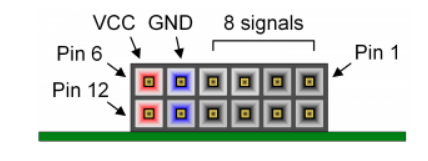
\includegraphics[width=0.5\textwidth]{figs/pmod_pins.png}
\end{center}

In the constraint file \verb|lab4/constrs/pynq-z1.xdc|, the following lines have been added.

\begin{minted}{tcl}
set_property -dict { PACKAGE_PIN Y18   IOSTANDARD LVCMOS33 } [get_ports { PMOD_OUT_PIN1  }]
set_property -dict { PACKAGE_PIN Y19   IOSTANDARD LVCMOS33 } [get_ports { PMOD_OUT_PIN2  }]
set_property -dict { PACKAGE_PIN Y16   IOSTANDARD LVCMOS33 } [get_ports { PMOD_OUT_PIN3  }]
set_property -dict { PACKAGE_PIN Y17   IOSTANDARD LVCMOS33 } [get_ports { PMOD_OUT_PIN4  }]
set_property -dict { PACKAGE_PIN U18   IOSTANDARD LVCMOS33 } [get_ports { PMOD_OUT_PIN7  }]
set_property -dict { PACKAGE_PIN U19   IOSTANDARD LVCMOS33 } [get_ports { PMOD_OUT_PIN8  }]
set_property -dict { PACKAGE_PIN W18   IOSTANDARD LVCMOS33 } [get_ports { PMOD_OUT_PIN9  }]
set_property -dict { PACKAGE_PIN W19   IOSTANDARD LVCMOS33 } [get_ports { PMOD_OUT_PIN10 }]
\end{minted}

These TCL commands set the pin mapping of the signals from our top-level module to the correct PMOD pins. We do not use pin 7 to 10 for now as our Pmod I2S only has 6 pins.

The DAC enables our board to output a high-fidelity stereo audio. It is a nicer alternative to the on-board audio output since we can stream audio data with up to 24-bit and two-channel (stereo) at high sampling rate using PCM (Pulse Code Modulation) scheme. On the other hand, the on-board audio can only play mono output. The Pmod I2S uses a \href{https://d3uzseaevmutz1.cloudfront.net/pubs/proDatasheet/CS4344-45-48_F2.pdf}{Cirrus Logic CS4344 D/A converter}. ``I2S'', also written I\textsuperscript{2}S, is the name of the interface format used to communicate with the chip.

\subsection{Interface Setup}

\begin{enumerate}
  \item Read the Pmod I2S reference manual carefully.
  \item Look over the CS4344 datasheet to reinforce what the reference manual said.
  \item If it helps, skim wider resources like the \href{https://en.wikipedia.org/wiki/I\%C2\%B2S}{Wikipedia \itwos{} article} to get a feel for what you're implementing.
  \item Also skim through \href{https://en.wikipedia.org/wiki/Pulse-code_modulation}{PCM} to understand how we want to store our audio data.
\end{enumerate}

The \itwos{} interface is a lot simpler than other common digital audio interfaces, like AC'97. Like AC'97, however, it requires us to generate very specific clocks for communication. Your \textbf{first task} in this part will be to generate the three requisite clock signals for the \itwos{} interface: the master clock \verb|MCLK|, a bit/serial clock \verb|SCLK|, and a left/right channel-select clock \verb|LRCK|. (That means that we will use an ``external'' \verb|SCLK| source for the CS4344.) These clocks are all derived from our 125 MHz system clock.

Note the special requirements on audio bit alignment to the clock edges, and on which bits are transmitted when. Your \textbf{second task} is to generate a bit counter that will track which bit of each sample to output for each bit clock.

The DAC chip allows us to select bit depth and sampling rate. For this lab, we will deal with audio data with a \textbf{bit depth of 16-bit}, and a \textbf{sampling rate of 44.1 KHz}. That means we have 44100 audio samples/frames per second which each frame is a 16-bit signed number in two's complement format. Therefore, a sample value is within a range of [-32768, 32767].

Figure \ref{fig:timing} summarizes timing for the interfaces. You can see the oddity in timing that the LSB of the last sample is sent on the \verb|LRCK| clock transition, and the MSB of the next sample is followed right after. You are encouraged to follow the spec to get the timing right. However, \textbf{it is not required} that you need to match this timing perfectly. Even if you do not follow exactly the timing specification, the sound generated from the Pmod chip is still comfortably audible (and if you look closely at Figure 7, Page 13 of the \href{https://d3uzseaevmutz1.cloudfront.net/pubs/proDatasheet/CS4344-45-48_F2.pdf}{Cirrus Logic CS4344 D/A converter} manual, all the bits of a frame actually fit in one channel, or half a period of the \verb|LRCK| clock).

\begin{figure}[H]
  \begin{center}
    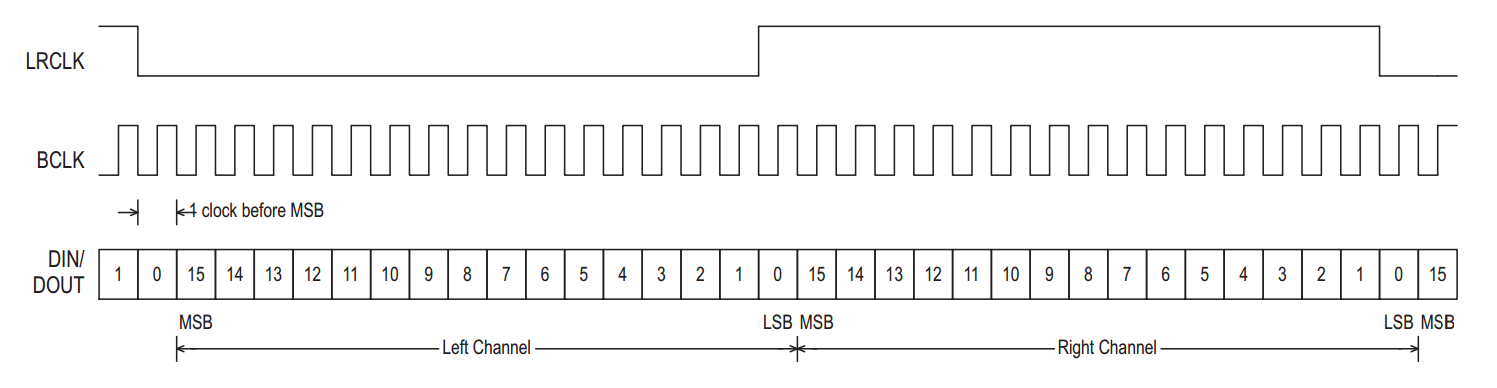
\includegraphics[width=6in]{figs/pmodi2s_timingdiagram.png}
    \caption{\itwos{} timing summary (credit: Texas Instruments)}
    \label{fig:timing}
  \end{center}
\end{figure}

In summary, to make your life easier when designing the I2S protocol, you can use the following suggestions.

\begin{enumerate}
  \item Ensure that (\verb|MCLK| clock rate / \verb|LRCK| clock rate) is an integer value as specified in the spec. \textbf{Use 512 for this lab}.
  \item Ensure that (\verb|LRCK| clock rate / \verb|SCLK| clock rate) is either 32 or 48. \textbf{Use 32 for this lab}.
  \item Ensure that \textbf{16 bits} of an audio frame is sent in one half period of the \verb|LRCK| clock starting from the MSB to the LSB. Send that frame again for the remaining half period of the \verb|LRCK| clock (i.e., we will be sending the same audio frame to both the left and right channel). You can send each bit at the rising edge of the \verb|SCLK| clock.
\end{enumerate}

The reason we want to keep the left and the right frames similar is to reduce the memory storage on the FPGA. You are, however, free to explore different settings to achieve good audio output. There are some testbenches provided to help you test the I2S interface implementation:

\verb|i2s_bit_serial_tb.v|: this testbench tests if you can send a sequence of bits from the input sample audio data starting from the MSB in successive cycles.

\verb|i2s_controller_tb.v|: this testbench tests if the ratios of the clock signals you generated match the spec. You should ensure that the ratios are integers (or very close to integers), otherwise you might not be able to generate the sound on the chip, or your sound might have some noise.

\subsection{Tone Generator}

In this section, we will build a circuit that generates a musical tone using a lookup-based approach. We use a simple Python script to create a sinusoidal wave with a frequency of 440 Hz, and sample it with a sampling rate of 44.1 kHz. The sample data is converted to 16-bit integers stored in our FPGA memory. In other words, the amount of memory needed for this tone is 44100 x 16 bits.

Your task is to complete the logic of \verb|lab4/src/z1top_tone_generator.v| so that it can play a 440 Hz tone. A ROM with the 440Hz-tone data has been instantiated for you. You need to figure out how to read the data from the ROM and interface with the I2S protocol to send the bit stream to the Pmod I2S correctly. It is expected that your design should be able to play a clean sound (minimum noise is acceptable). You can compare your 440Hz - tone generator circuit with this \href{https://www.szynalski.com/tone-generator}{Online Tone Generator}. You can also use the Python script in \verb|lab4/script/tone_gen.py| to generate different tones for testing.

\begin{minted}{python}
# args: {frequency} {duration} {number of samples}
python3 tone_gen.py 440 2 65536
\end{minted}

You can use the \verb|z1top_tone_generator_tb.v| testbench to verify if your top-level module generates correct audio as in \verb|tone_440_data_bin.mif|. The testbench expects correct audio bits at every rising edge of the serial clock (\verb|PMOD_PIN_3|). You may want to change it depending on how you want to implement the I2S interface. The testbench may take a few minutes to complete, so you should abort it as long as you spot any mismatches' messages.
 
\subsection{Multi-tone Player (Optional)}

In this section, we will build a circuit that can play more than one tone. It's entirely up to you how many tones you want to play, just note that the FPGA memory resource is scarce. You might even want to use both LUTRAMs and BRAMs to store tone data. It might also take longer to generate a bitstream if you try to exhaust the resource on the FPGA. Each tone is controlled by one button on the board (you can use a combination of buttons and switches to expand the number of tones you want to support). Press a button, and the tone will play for a fixed time duration of your own choice in your design (a few seconds). It's like a piano, but we are limited in the number of tones and keys we want to play.

You should update the file \verb|lab4/src/z1top_multi_tones.v| to implement the logic. This part is optional.

\subsection{Music player}

In this section, we will build a circuit that play a short musical excerpt from "The Blue Danube". The music file has been converted to a hex mif file for initializing your ROM

\verb|lab4/src/The_Blue_Danube.mif|

with 262144 audio samples. Therefore, our memory requirement is 262144 x 16 bits. This would utilize around 262144 / 1024 = 256 blocks of 18Kb RAMs on our FPGA (91\% BRAM utilization). Since the sampling rate is 44.1 kHz, the music only lasts for 262144 $\times$ 1 / 44100 or around 6 seconds!

You should update the file \verb|lab4/src/z1top_music_player.v| to play the music stored in our BRAMs. Additionally, you should build a control logic using FSM for the music as follows.
\begin{enumerate}
  \item The music should play for around 6 seconds and stop.
  \item SWITCHES[0] == 1, BUTTONS[0] is pressed: play/pause the music.
  \item SWITCHES[0] == 1, BUTTONS[1] is pressed: increase the tempo of the music. You can do this by, for example, skipping a frame.
  \item SWITCHES[0] == 1, BUTTONS[2] is pressed: decrease the tempo of the music. You can do this by, for example, playing a frame twice.
  \item SWITCHES[0] == 1, BUTTONS[3] is pressed: reset the player. The music player should operate normally afterwards.
  \item SWITCHES[0] == 0, BUTTONS[0] is pressed: increase the volume of the music. You can try increasing the ROM rdata value.
  \item SWITCHES[0] == 0, BUTTONS[1] is pressed: decrease the volume of the music. You can try decreasing the ROM rdata value.
\end{enumerate}

The amount of change when increasing/decreasing the tempo and increasing/decreasing the volume is left for you to decide.

If you are confused, or unsure how to move on in any parts above, please do not hesitate to discuss with TA for hints.

In this lab, we have attempted to push the PYNQ board to its limit for the task of music streaming. The amount of on-chip storage is clearly not enough to play something like a song. We could, however, leverage the off-chip DRAM memory with a capacity of 512MB, but that would require our logic to communication with the ARM processor since it acts as a memory controller to the off-chip DRAM. In addition, off-chip memory access is unpredictable and we would need some buffering scheme to ensure steady music streaming. Another viable path is to build an audio synthesizer that generates music from a list of notes in real time. Those are beyond the scope of our lab for now.

\newpage
\section{Lab Deliverables (due: 11.59PM, Feb 27th, 2020)}
\subsection{Lab Checkoff}
To checkoff for this lab, have these things ready to show the TA:
\begin{enumerate}
  \item Demonstrate working accumulation designs with ASYNC\_ROM and SYNC\_ROM.
  \item Demonstrate that your design can play a 440Hz-tone via the Pmod I2S.
  \item Demonstrate that your design can play different tones via the Pmod I2S (more than one). This part is optional.
  \item Demonstrate that your design can play some short music and that you can pause/resume, increase/decrease the tempo, and increase/decrease the volume via the Pmod I2S.
\end{enumerate}

\subsection{Lab Report}\label{sec:labreport}

There is no report required for this lab. Focus on getting things right, and make sure you adopt the EECS151-Spring20 policy for register and memory module instantiations.

\newpage
\section*{Ackowlegement}
This lab is the result of the work of many EECS151/251 GSIs over the years including:
\begin{itemize}
\item Sp12: James Parker, Daiwei Li, Shaoyi Cheng
\item Sp13: Shaoyi Cheng, Vincent Lee
\item Fa14: Simon Scott, Ian Juch
\item Fa15: James Martin
\item Fa16: Vighnesh Iyer
\item Fa17: George Alexandrov, Vighnesh Iyer, Nathan Narevsky
\item Sp18: Arya Reais-Parsi, Taehwan Kim
\item Fa18: Ali Moin, George Alexandrov, Andy Zhou
\item Sp19: Christopher Yarp, Arya Reais-Parsi
\item Fa19: Cem Yalcin, Rebekah Zhao, Ryan Kaveh, Vighnesh Iyer
\end{itemize}

\end{document}
